\chapter{Neural Circuits}

Nervous systems are not merely a collection of neurons. Rather, neurons of many different varieties are arranged in specific neural \textit{circuits}, which form the large-scale structures outlined in Chapter \ref{chap: anatomy}. The circuit-level study of nervous systems offers a promising direction for understanding both the function and implementation of brain areas. Perhaps by understanding the basic design principles of \textit{canonical} circuits, we may be able to identify a core set of computational operations utilized by the brain.

The brain is made up of specialized areas, which interconnect in specific ways. Each area receives \textit{input fibers}, which form synapses on the cells within that area. The incoming signal, perhaps after some processing, is then sent to other areas via a set of neurons called \textit{principle, relay}, or \textit{projection} neurons. Other cells are only involved in the processing within the area and are instead referred to as \textit{intrinsic, local,} or \textit{inter-}neurons. 


\section{Circuit Motifs}

\subsection{Mutual Inhibition}


\subsection{Feedforward Inhibition}







\section{Retinal Circuits}


\section{Cerebellar Circuits}


\section{Thalamocortical Circuits}

Thalamus is the `relay' for cortical inputs. It is divided into (1) \textbf{first-order} and (2) \textbf{higher-order} nuclei. First-order nuclei receive inputs from sensory organs and project to primary sensory cortical areas. Higher-order nuclei receive inputs from cortex (specifically layer 5b) and project back to cortex. These circuits area shown in Figure \ref{fig: thalamocortical circuits}. Intriguingly, there are then at least two types of pathways within cortex: direct connections between cortical areas and indirect connections through thalamus. Furthermore, no connections have been identified between higher-order thalamic relay cells. Additionally, the cortical layer 5b cells that project down to higher-order thalamus have branching axons that also send information to sub-cortical motor centers.

\begin{figure*}[h!]
    \centering
    \begin{subfigure}[t]{0.5\textwidth}
        \centering
        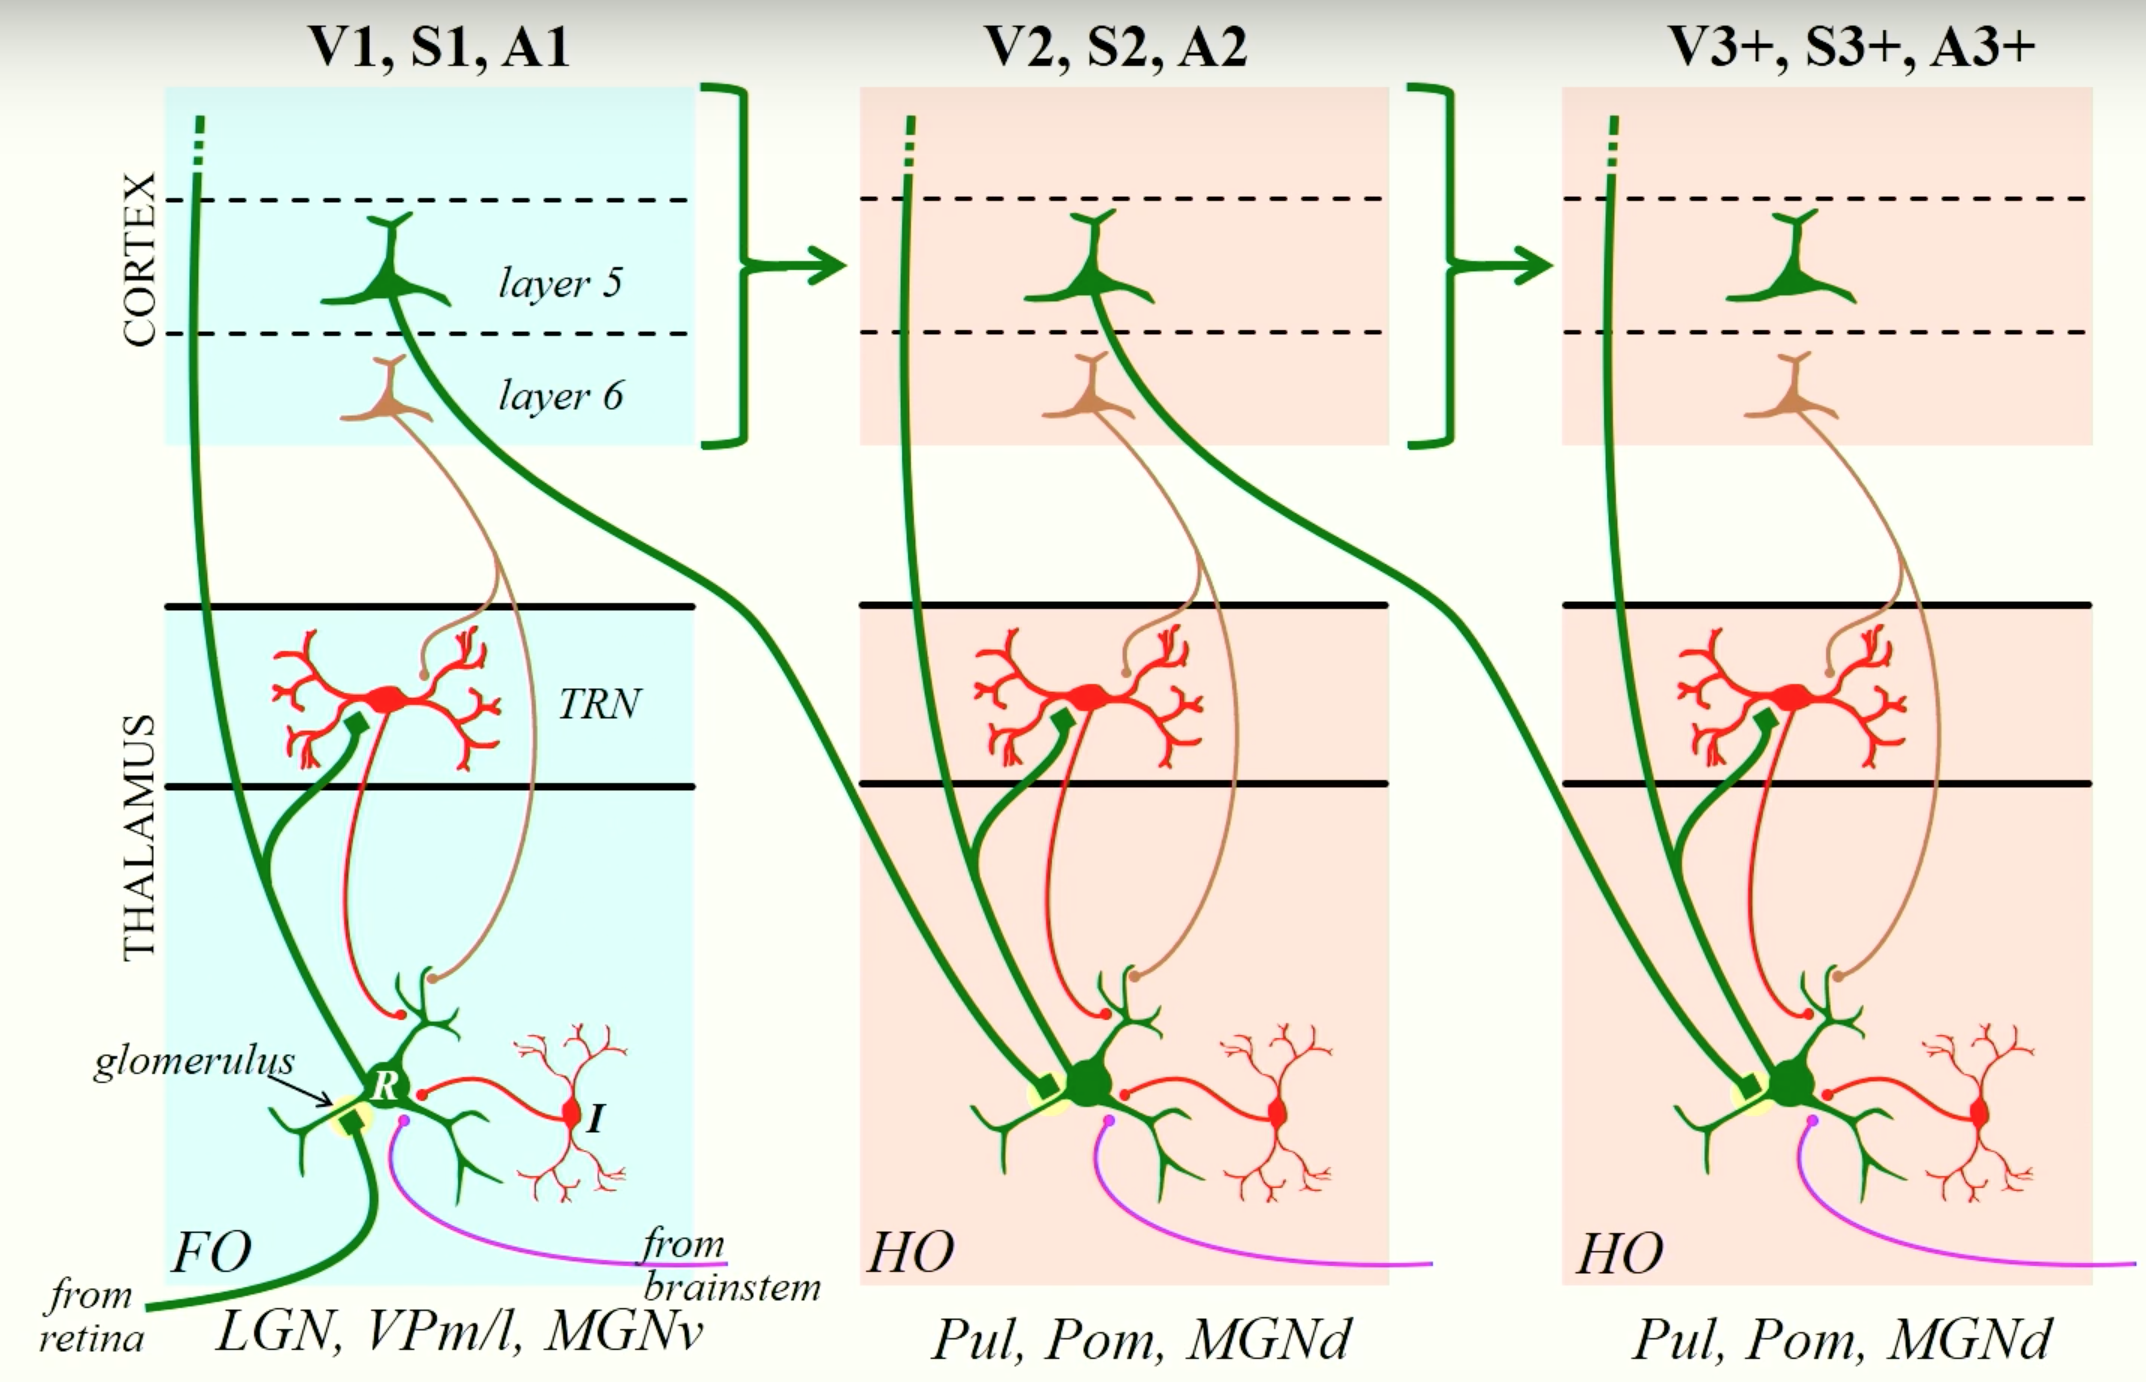
\includegraphics[width=\textwidth]{images/neuroscience/thalamocortical_circuits.png}
        \caption{ }
        \label{fig: thalamocortical circuits}
    \end{subfigure}%
    ~ 
    \begin{subfigure}[t]{0.5\textwidth}
        \centering
        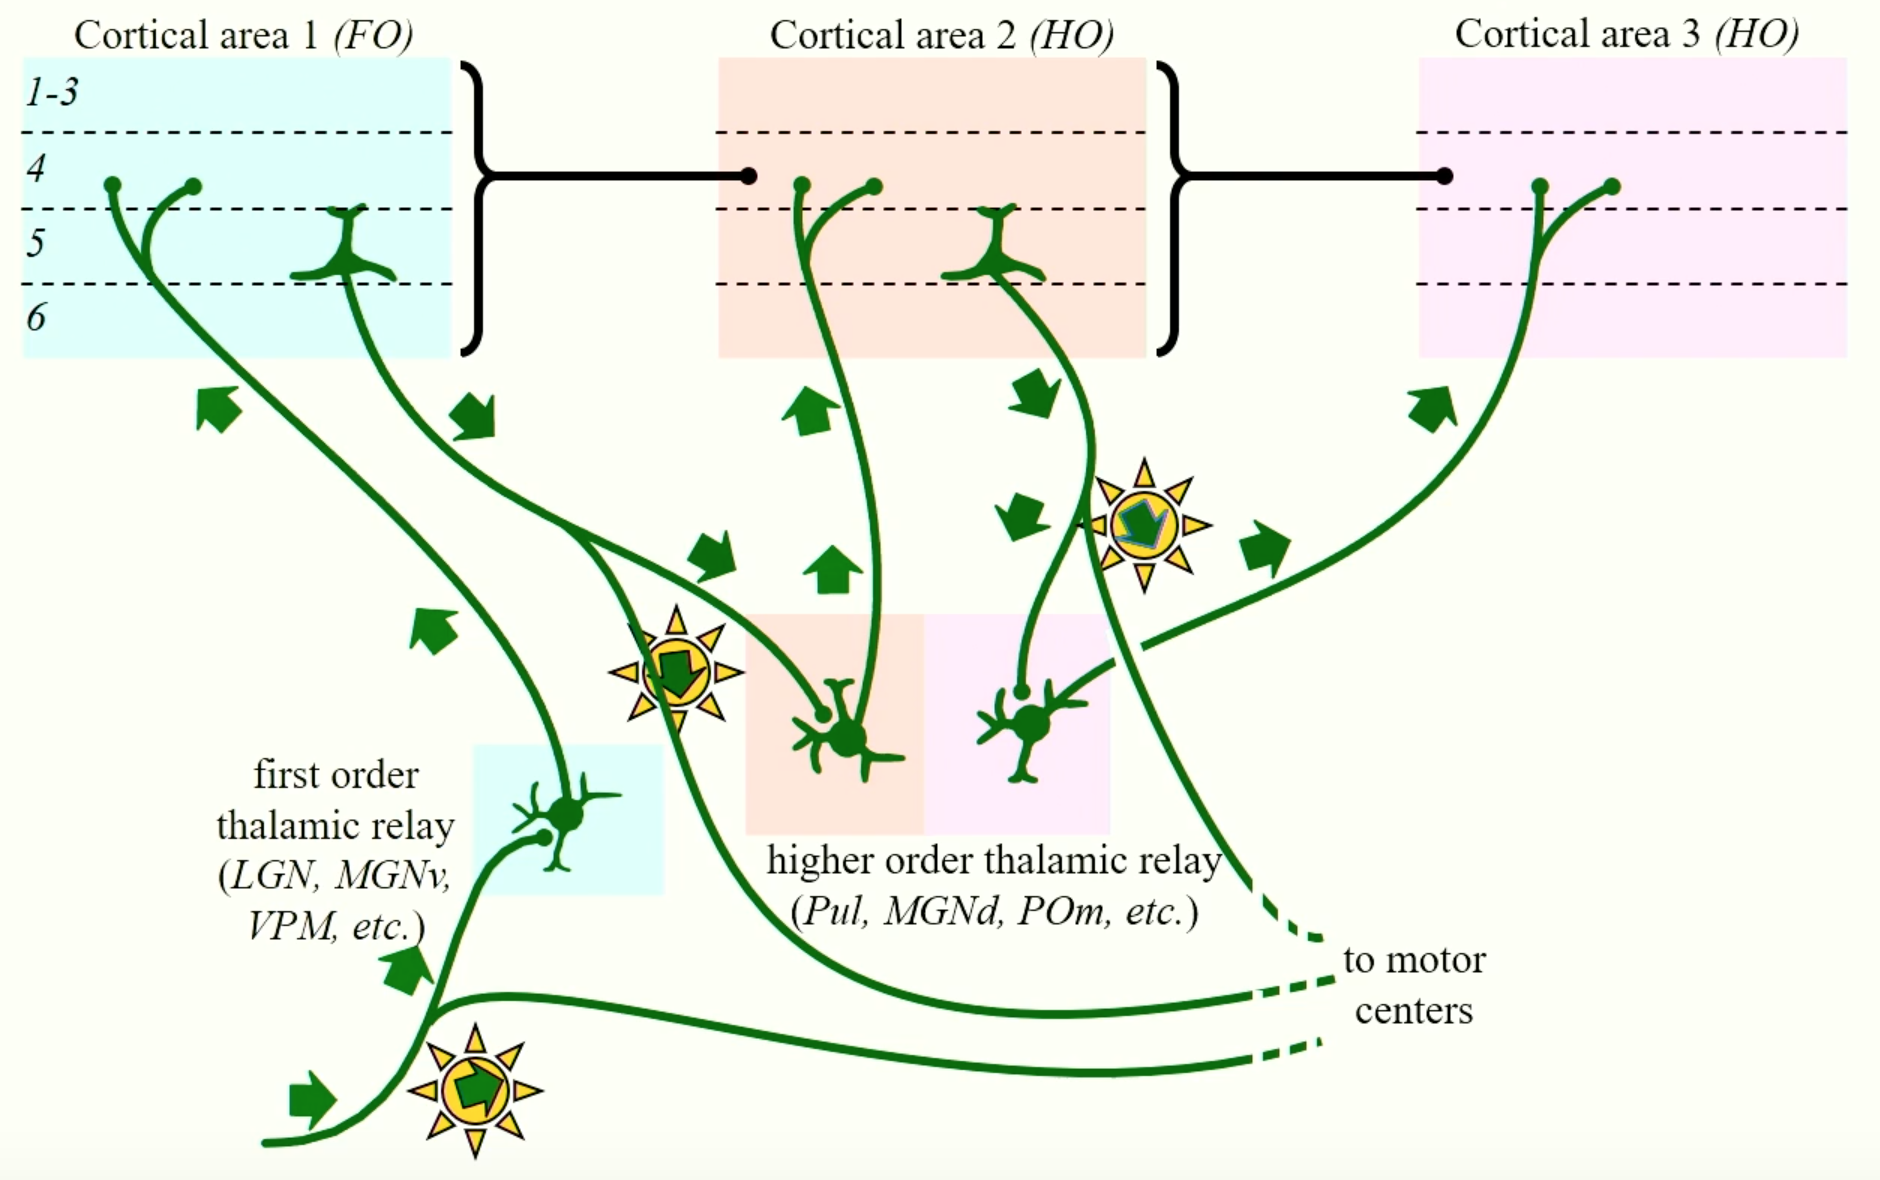
\includegraphics[width=\textwidth]{images/neuroscience/thalamus_branching_axons.png}
        \caption{ }
        \label{fig: thalamus branching axons}
    \end{subfigure}
    \caption{(\textbf{a}) Basic circuit diagram of first-order (left) and higher-order (center, right) thalamocortical circuits across multiple sensory modalities. (\textbf{b}) Cortical cells that project to thalamus often have branching axons that also project to sub-cortical motor centers. Reproduced from S. Murray Sherman.}
\end{figure*}


\section{Neocortical Circuits}

A review of various experimental findings on cortical circuits is presented in \cite{harris2015neocortical}. While there are differences in cortical structure and activity across different areas and species, many cortical circuit properties are conserved. \cite{harris2015neocortical} therefore argues that these differences are \textit{quantitative} rather than \textit{qualitative}, arising from differences in gene expression and inputs. They refer to these slight differences on a main conserved architecture as \textit{serial homology}. The primary categorization of neocortical neurons is between excitatory cells (EC), which constitute roughly $80\%$ of neurons, and interneurons, which constitute the remaining $20\%$.  

A somewhat more simplistic view, with a focus on predictive coding, is presented in \cite{bastos2012canonical}.

\subsubsection{Excitatory Cells}

Excitatory cells are classified into three main categories:
\begin{itemize}
	\item \textbf{intratelencephalic (IT) neurons}: Found in layers 2-6 and project axons only within the telecephalon (neocortex, striatum, and corticoid structures such as amygdala and claustrum). They are the only ECs that project to contralateral cortex. There are many distinct subclasses of IT cells, such as those found in L4.
	\item \textbf{pyramidal tract (PT) neurons}: These are large pyramidal neurons found in layer 5B that project to subcerebral targets including brain stem, spinal cord and midbrain, as well as thalamus and striatum. 
	\item \textbf{corticothalamic (CT) neurons}: Found in layer 6 and project primarily to ipsilateral thalamus.
\end{itemize}
Morphologies of these cell types are shown in Figure \ref{fig: cortical morphologies}. It should be noted that all class of ECs form recurrent connections with local neurons of the same class. Across classes, however, the connectivity is asymmetric, which has led to the hypothesis of a sequential circuit organization. This sequence is typically understood in terms of
$$ \text{thalamus} \rightarrow \text{L4 IT neurons} \rightarrow \text{Other IT neurons} \rightarrow \text{PT neurons},$$
with the role of CT neurons within the circuit still largely unknown. 

\begin{figure}[h]
    \centering
    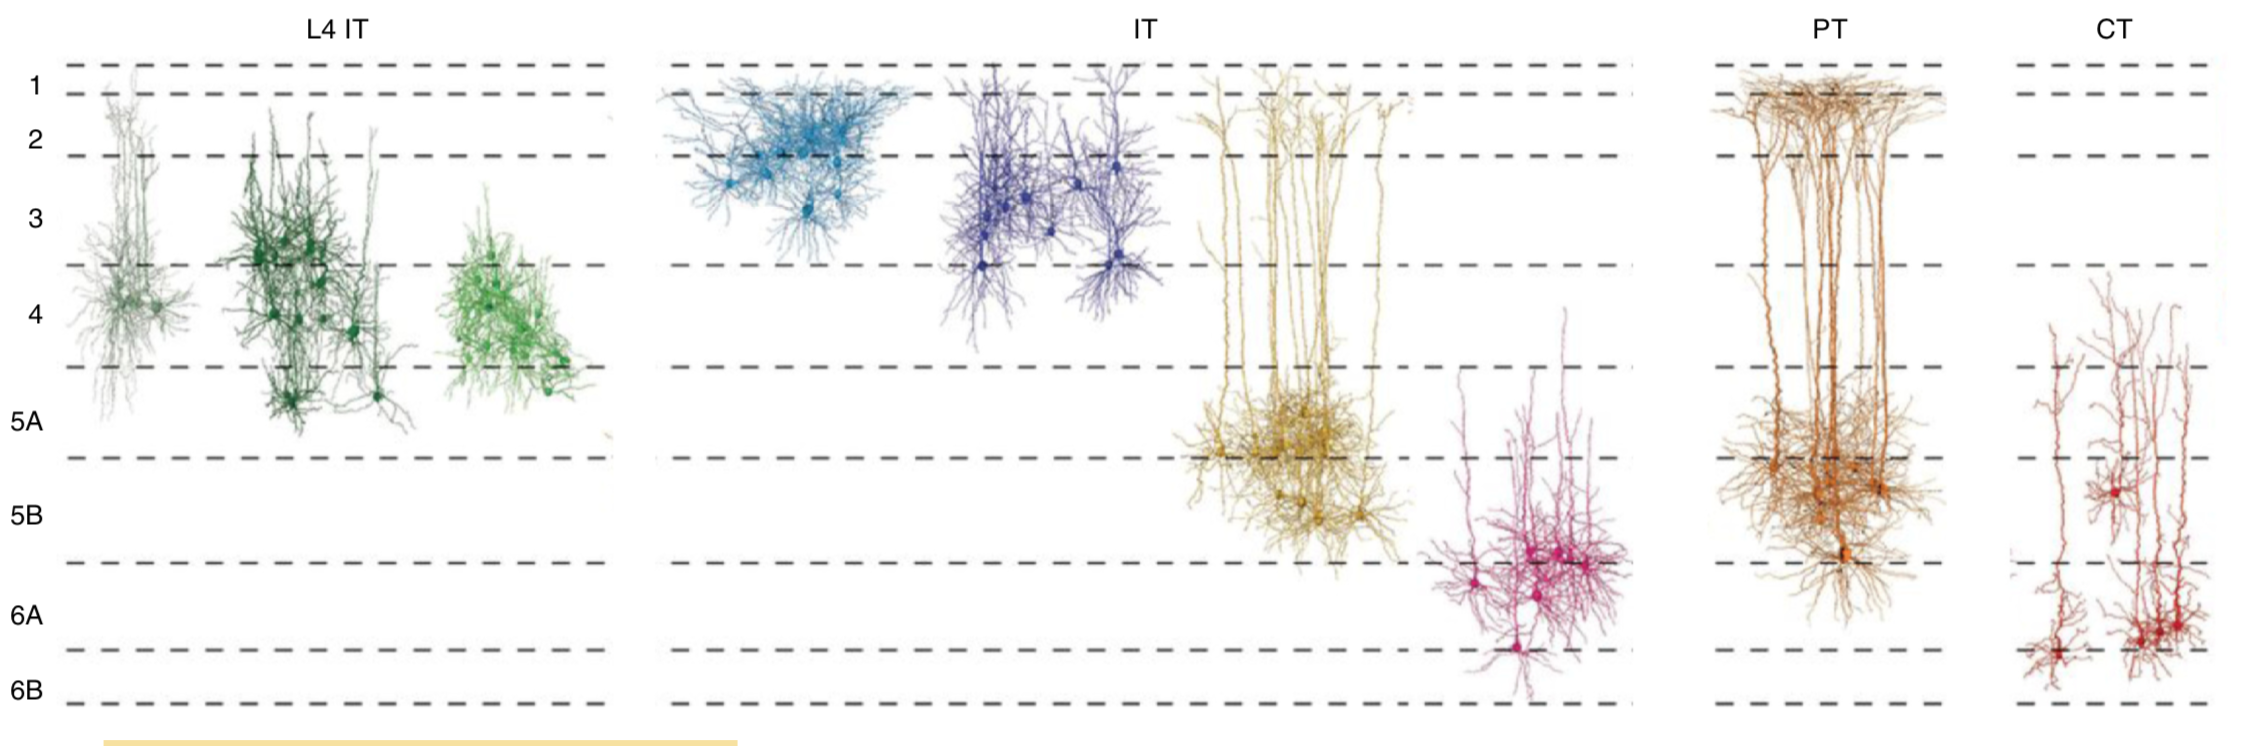
\includegraphics[width=\textwidth]{images/neuroscience/cortical_morphologies.png}
    \caption{Morphologies of various classes of excitatory cells in neocortex. Reproduced from \cite{harris2015neocortical}.}
    \label{fig: cortical morphologies}
\end{figure}

Most of the subcortical inputs to the cortex arise from thalamus and are roughly divided into ``core" and ``matrix" connections. The core relay neurons carry rapid sensory or motor information and are located in primary relay nuclei. These axons tend to form topographic connections in L4 or primary sensory areas. The matrix relay neurons are not well understood, but are typically found in higher order nuclei and project to L1 (and sometimes other layers) of one or more cortical areas. The core-matrix distinction applies most directly to primary sensory areas, but is also found in motor areas and possibly other areas. Higher order sensory cortex, for instance, receives predominantly matrix-type thalamocortical (TC) connections. 

L4 neurons are a special case of IT neurons. They project asymmetrically to L2/3 and L5, and are therefore considered ``upstream" of other circuit components. There are many morphological subclasses of L4 IT neurons, but they largely have similar circuit properties. Layer 4 is enlarged in primary sensory areas, so L4 neurons are thought to be specialized for sensory processing, with different sensory areas tuned appropriately. In higher-order sensory areas, L4 receives input from thalamus as well as lower areas of cortex. Although motor areas appear to lack a well defined L4, they may contain L4 type cells. 

Other IT neurons receive input from L4 neurons and TC connections. Their outputs project to distant neocortical and striatum areas as well as locally to PT and CT neurons. L2 IT neurons receive matrix-type TC input and inputs from L5A and L4. L3 IT neurons receive similar inputs, with the addition of core-type TC inputs. These neurons tend to exhibit sparse firing and project to L5. The L5 IT neurons tend to be reciprocally connected to L2/3 and also have broad range connections, particularly to striatum. L6 IT neurons are less studied but tend to make distant connections. 

PT neurons receive cortical (L2/3) and TC (core-type) input and project to specialized subcortical areas, such as spinal or tectal areas. They also make connections with ipsilateral cortex and thalamus. They tend to display bursting firing patterns, which provide a ``dense code." This is perhaps an information-theoretic adaptation to broadcast cortical output through a small number of channels. 

CT neurons are found in L6, and tend to receive input from higher-order cortical areas, as well as some input from thalamus. Their projections to thalamic areas are slow and weak, so they are often considered as modulators instead of drivers. It is thought that CT neurons may integrate long-range cortical inputs to modulate TC activity, acting as a sort of gain control. 

\begin{figure}[h]
    \centering
    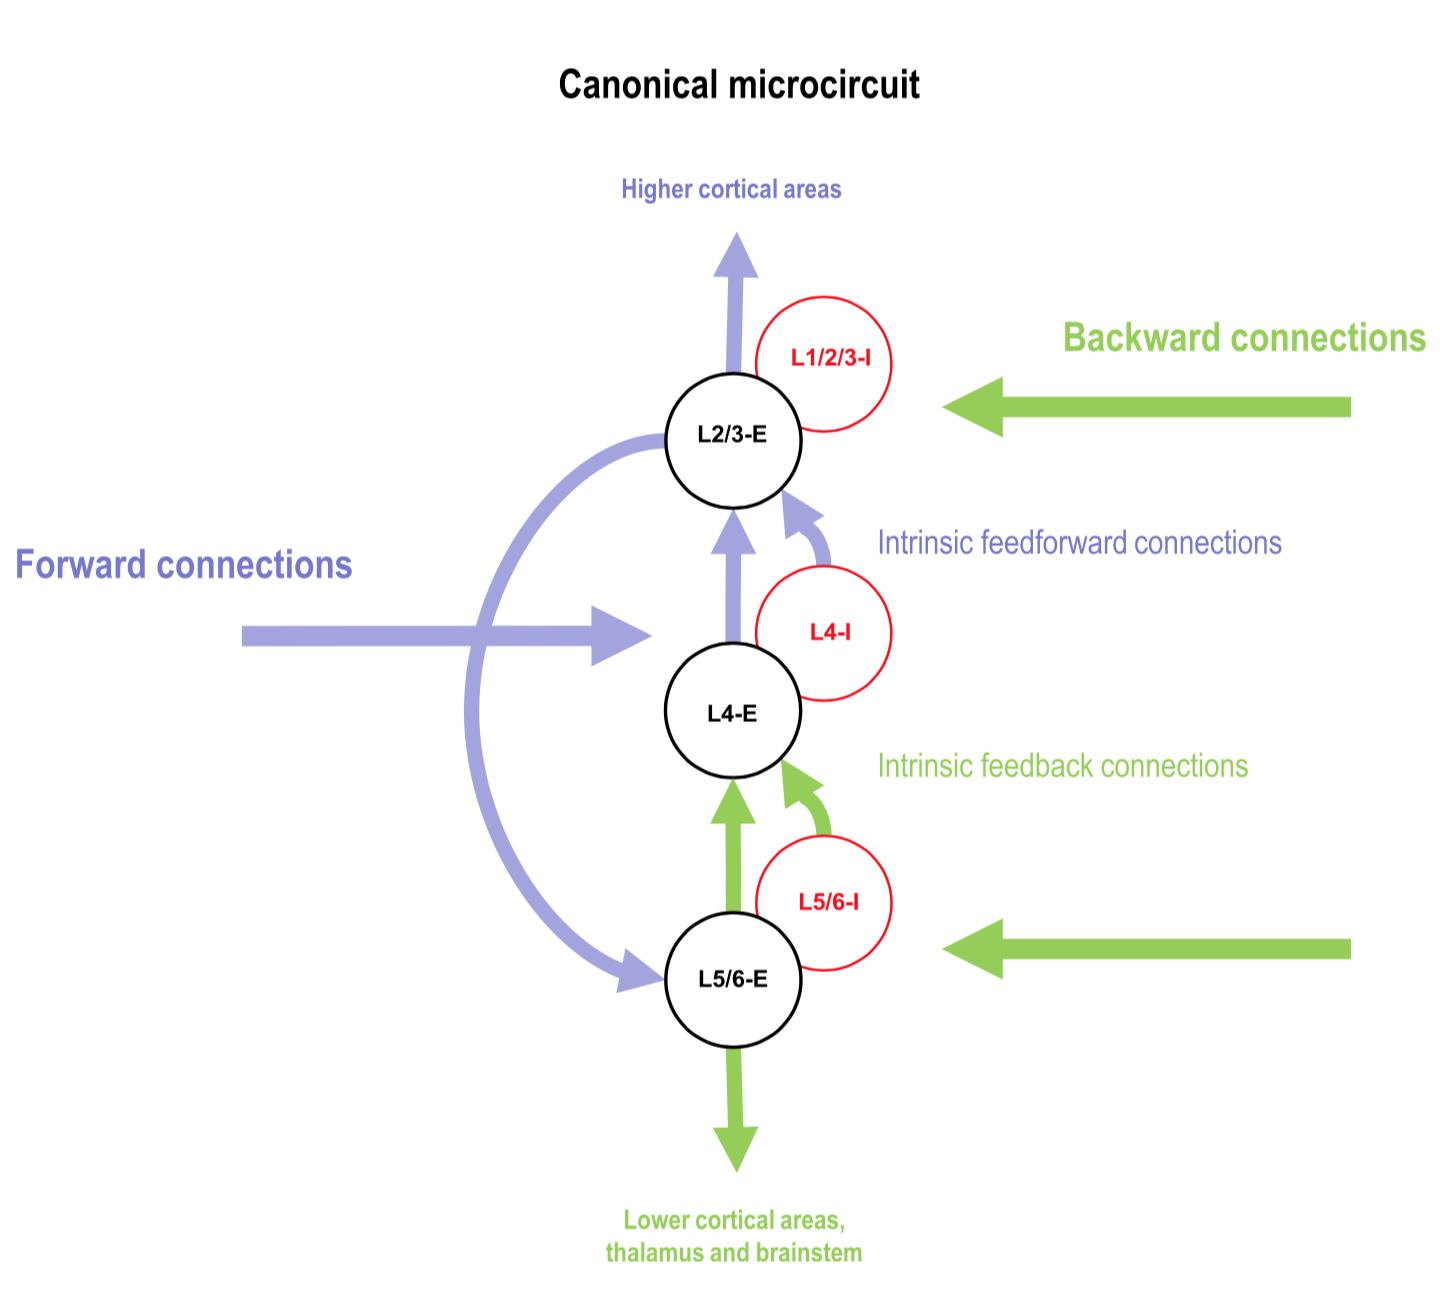
\includegraphics[width=0.75\textwidth]{images/neuroscience/pc_connectivity.png}
    \caption{Connectivity diagram for a cortical microcircuit. Reproduced from \cite{bastos2012canonical}.}
    \label{fig: pc connectivity}
\end{figure}

\subsubsection{Interneurons}

Cortical interneurons are categorized into three classes based on gene expression:
\begin{itemize}
	\item \textbf{Pvalb}
	\item \textbf{Sst}
	\item \textbf{Htr3a}
\end{itemize}
Interneurons contain many subclasses, which inhibit various local ECs and other interneurons. These inhibitory circuits may mediate diverse control of cortical processing during behavior, at least partially contributing to the quantitative differences between cortical circuits that perform different computations, yet have similar qualitative architectures. 

